\chapter{Classes: Introduction}

\section{Grouping Related Items into Objects}

The physical world is made up of materials such as \textbf{wood}, \textbf{metal}, \textbf{plastic}, and \textbf{fabric}.
To make sense of it, we group materials into higher-level concepts such as \textit{chairs}, \textit{tables}, and \textit{televisions}.
Similarly, in programming, we group lower-level data and functions into \textbf{objects}.

\begin{quote}
An \textbf{object} is a bundle of data (variables) and the operations (methods) that act on that data.
\end{quote}

\subsection*{Example: Thinking in Objects}

\begin{center}
\begin{tabular}{|l|l|}
\hline
\textbf{Object} & \textbf{Operations (Methods)} \\
\hline
Chair & \texttt{sit()} \\
Couch & \texttt{sit()}, \texttt{lie\_down()} \\
Drawer & \texttt{put\_item()}, \texttt{take\_item()} \\
\hline
\end{tabular}
\end{center}

Objects let us think about the world in terms of \emph{what things do}, rather than what they are made of.

\subsection*{Participation Discussion}
\begin{itemize}
  \item What real-world object do you interact with daily that could be modeled as a class?
  \item What are its attributes (data) and behaviors (methods)?
\end{itemize}

\subsection{Programs Viewed as Objects}

A program consists of variables and functions, but object-oriented programming encourages us to group related data and actions together.

\begin{center}
\begin{tabular}{|l|l|}
\hline
\textbf{Object Type} & \textbf{Possible Actions} \\
\hline
Restaurant & \texttt{set\_name()}, \texttt{add\_cuisine()}, \texttt{add\_review()} \\
Hotel & \texttt{set\_name()}, \texttt{add\_amenity()}, \texttt{add\_review()} \\
\hline
\end{tabular}
\end{center}

\noindent
\textit{By organizing code this way, we create programs that are easier to read, extend, and maintain.}

\section{Abstraction and Information Hiding}

Abstraction occurs when we use an interface (like an oven’s knob) to hide complex inner details (like heating elements).

\begin{quote}
Objects simplify complexity by hiding details and exposing only essential operations.
\end{quote}

\textbf{Example:}
\begin{center}
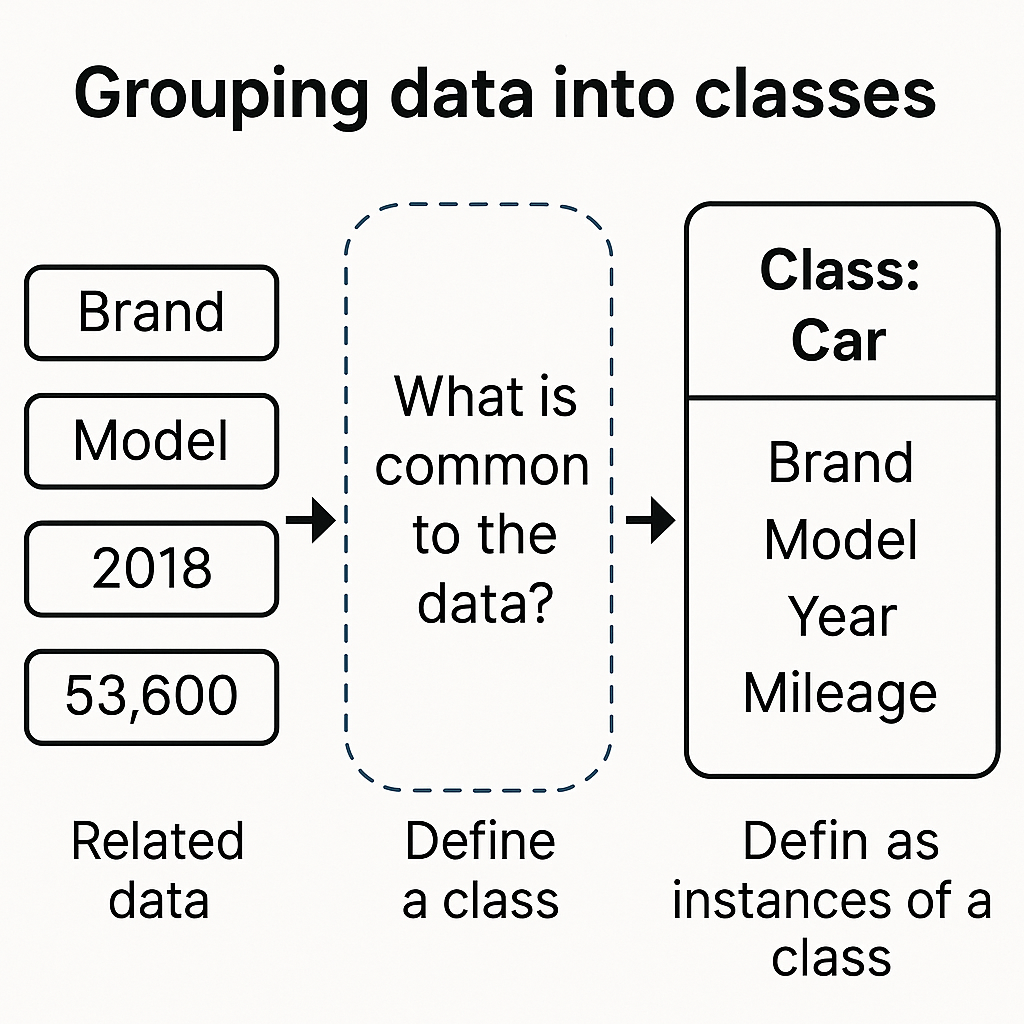
\includegraphics[width=0.8\textwidth]{../images/oven_abstraction_example.png}
\end{center}

\begin{itemize}
  \item A car hides the details of its engine behind a steering wheel, pedals, and a dashboard.
  \item A Python object hides the details of its data, offering you methods like \texttt{.append()} or \texttt{.lower()}.
\end{itemize}

\section{Built-in Objects in Python}

Python automatically provides built-in objects, like:
\begin{itemize}
  \item \texttt{str} — string data type (ex: \texttt{"Hello"})
  \item \texttt{int} — integer data type (ex: \texttt{42})
\end{itemize}

\textbf{Example:}
\begin{verbatim}
s1 = "Hello!"
print(s1.upper())   # Output: HELLO!
i1 = 130
print(i1.bit_length())  # Output: 8
\end{verbatim}

\textit{Even built-in types are objects with data and methods!}

\section*{Reflection Questions}

\begin{enumerate}
  \item What does it mean to say “a program is made of objects”?
  \item Why does abstraction make code easier to understand?
  \item Can you think of three real-world items that could become classes in code?
\end{enumerate}

